\documentclass{article}\usepackage[]{graphicx}\usepackage[]{color}
%% maxwidth is the original width if it is less than linewidth
%% otherwise use linewidth (to make sure the graphics do not exceed the margin)
\makeatletter
\def\maxwidth{ %
  \ifdim\Gin@nat@width>\linewidth
    \linewidth
  \else
    \Gin@nat@width
  \fi
}
\makeatother

\definecolor{fgcolor}{rgb}{0.345, 0.345, 0.345}
\newcommand{\hlnum}[1]{\textcolor[rgb]{0.686,0.059,0.569}{#1}}%
\newcommand{\hlstr}[1]{\textcolor[rgb]{0.192,0.494,0.8}{#1}}%
\newcommand{\hlcom}[1]{\textcolor[rgb]{0.678,0.584,0.686}{\textit{#1}}}%
\newcommand{\hlopt}[1]{\textcolor[rgb]{0,0,0}{#1}}%
\newcommand{\hlstd}[1]{\textcolor[rgb]{0.345,0.345,0.345}{#1}}%
\newcommand{\hlkwa}[1]{\textcolor[rgb]{0.161,0.373,0.58}{\textbf{#1}}}%
\newcommand{\hlkwb}[1]{\textcolor[rgb]{0.69,0.353,0.396}{#1}}%
\newcommand{\hlkwc}[1]{\textcolor[rgb]{0.333,0.667,0.333}{#1}}%
\newcommand{\hlkwd}[1]{\textcolor[rgb]{0.737,0.353,0.396}{\textbf{#1}}}%
\let\hlipl\hlkwb

\usepackage{framed}
\makeatletter
\newenvironment{kframe}{%
 \def\at@end@of@kframe{}%
 \ifinner\ifhmode%
  \def\at@end@of@kframe{\end{minipage}}%
  \begin{minipage}{\columnwidth}%
 \fi\fi%
 \def\FrameCommand##1{\hskip\@totalleftmargin \hskip-\fboxsep
 \colorbox{shadecolor}{##1}\hskip-\fboxsep
     % There is no \\@totalrightmargin, so:
     \hskip-\linewidth \hskip-\@totalleftmargin \hskip\columnwidth}%
 \MakeFramed {\advance\hsize-\width
   \@totalleftmargin\z@ \linewidth\hsize
   \@setminipage}}%
 {\par\unskip\endMakeFramed%
 \at@end@of@kframe}
\makeatother

\definecolor{shadecolor}{rgb}{.97, .97, .97}
\definecolor{messagecolor}{rgb}{0, 0, 0}
\definecolor{warningcolor}{rgb}{1, 0, 1}
\definecolor{errorcolor}{rgb}{1, 0, 0}
\newenvironment{knitrout}{}{} % an empty environment to be redefined in TeX

\usepackage{alltt}
\usepackage{amsmath, amssymb}
\IfFileExists{upquote.sty}{\usepackage{upquote}}{}
\begin{document}
%\SweaveOpts{concordance=TRUE}

\begin{knitrout}
\definecolor{shadecolor}{rgb}{0.969, 0.969, 0.969}\color{fgcolor}\begin{kframe}


{\ttfamily\noindent\itshape\color{messagecolor}{\#\# Registering fonts with R}}

{\ttfamily\noindent\itshape\color{messagecolor}{\#\# Package "{}fontcm"{} already installed.}}

{\ttfamily\noindent\itshape\color{messagecolor}{\#\# Registering font package "{}fontcm"{} with fonts.}}

{\ttfamily\noindent\itshape\color{messagecolor}{\#\# Font package "{}fontcm"{} already registered in fonts database.}}

{\ttfamily\noindent\itshape\color{messagecolor}{\#\# \\\#\# Attaching package: 'dplyr'}}

{\ttfamily\noindent\itshape\color{messagecolor}{\#\# The following objects are masked from 'package:plyr':\\\#\# \\\#\#\ \ \ \  arrange, count, desc, failwith, id, mutate, rename, summarise,\\\#\#\ \ \ \  summarize}}

{\ttfamily\noindent\itshape\color{messagecolor}{\#\# The following objects are masked from 'package:stats':\\\#\# \\\#\#\ \ \ \  filter, lag}}

{\ttfamily\noindent\itshape\color{messagecolor}{\#\# The following objects are masked from 'package:base':\\\#\# \\\#\#\ \ \ \  intersect, setdiff, setequal, union}}\end{kframe}
\end{knitrout}


\section{Description}
The symetric random walk will be described in this document (Mt). it covers the theory of "Stochastic Calculus for finance" Tome 2 chapter 3 section 1.

The construction of the random walk depend on the evolution of a random variable $X_i$. The previous RV can take two value at each time, like tossing a coin. $X_i$ can take the value 1 or -1.

\begin{equation}
 \label{eq:Xi}
X_i = 
\left \{{
  \begin{array}{c} 1 \\ -1 \end{array}
  }\right .
\end{equation}
 
The Symetric Random Walk is constructed by summing up the different outcome of the random variable $X_i$ from $k$ experiments:

\begin{equation}
\label{eq:SRW}
M_k = 
\sum_{j=1}^k X_j
\end{equation}

In the following lines of code, $X_i$ is randomly difined. The variable $k$ ensure to have a sufficent number of periods to further generate the scaled random walk.
It refers to the $k$ of equation~\ref{eq:SRW}.
$p$ and $q$ are the probability measure, respectively $p$ chance to get value 1 and $q$ chance to get -1 from random variable $X_i$.

 


After creating the random variable $X_i$ it suffices to add up all the differente output we get from time 1 up to $k$ to get a specific Symetric Random Walk.

The following outcome present a randomly generated 300 steps symmetric random walk.

\begin{table}[h]

\caption{300 steps Symmetric Random Walk}
\end{table}


\begin{figure}[!h]
\begin{center}

\begin{knitrout}
\definecolor{shadecolor}{rgb}{0.969, 0.969, 0.969}\color{fgcolor}
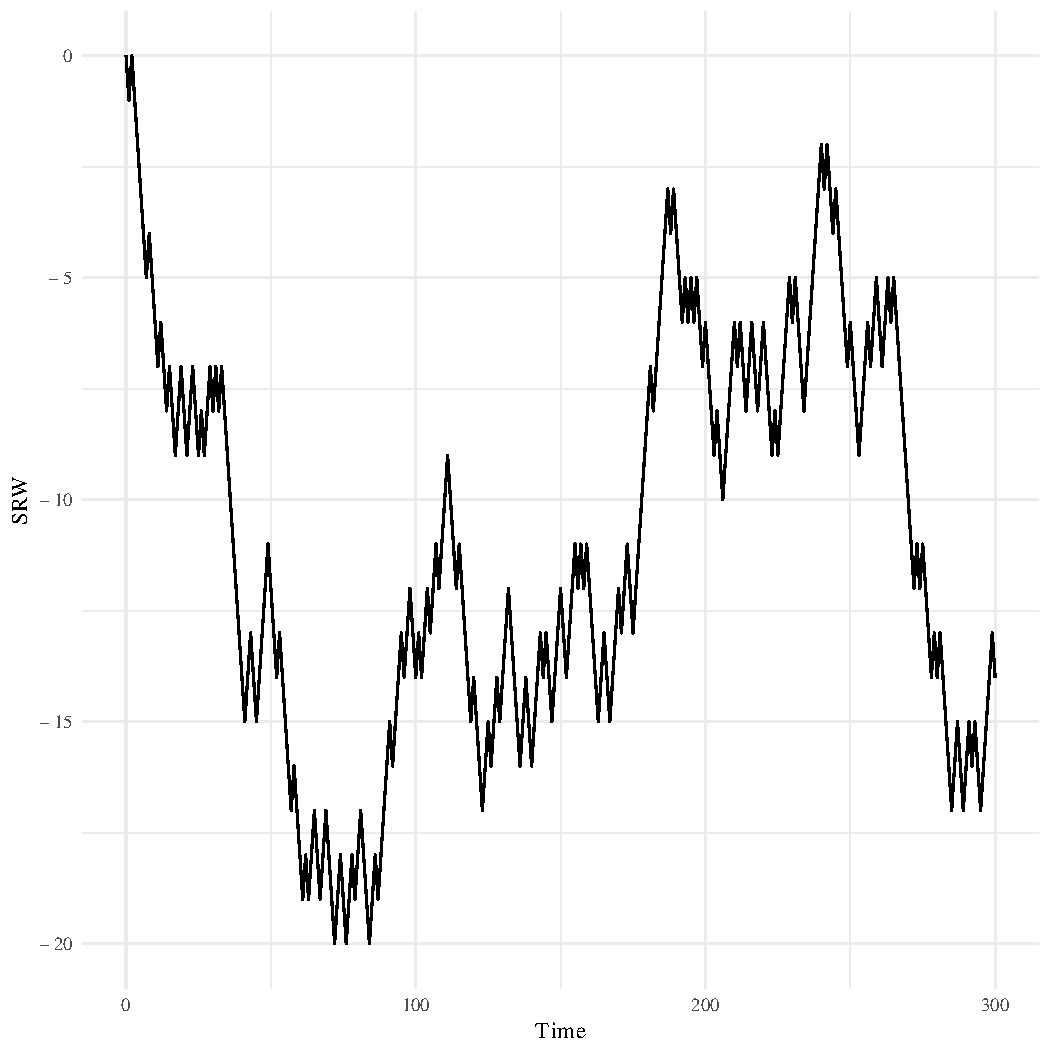
\includegraphics[width=1\linewidth]{figure/unnamed-chunk-4-1} 

\end{knitrout}


\end{center}
\caption{Symmetric Random Walk}
\end{figure}

\begin{kframe}
\begin{alltt}
\hlcom{# Because squared matrix dim(y) = dim(x):}
\hlstd{dim_x} \hlkwb{<-} \hlstd{dim_y} \hlkwb{<-} \hlnum{1}\hlopt{:}\hlstd{(k} \hlopt{+} \hlnum{1}\hlstd{)} \hlcom{# from 1 to k+1 because we start to time zero nonrandom which equal to zero}
\hlcom{# Create the symmetric random walk distribution:}
\hlcom{# ifelse is vectorized and therefore is consistent with the using of outer which accept only vectorized function.}
\hlstd{Mk} \hlkwb{<-} \hlkwd{outer}\hlstd{(dim_x,}
           \hlstd{dim_y,}
           \hlkwc{FUN}\hlstd{=}\hlkwa{function}\hlstd{(}\hlkwc{r}\hlstd{,}\hlkwc{c}\hlstd{)\{}\hlkwd{ifelse}\hlstd{(c}\hlopt{>=}\hlstd{r, (c}\hlopt{-}\hlstd{r)} \hlopt{-} \hlstd{(r}\hlopt{-}\hlnum{1}\hlstd{),} \hlnum{NA_integer_}\hlstd{)\})}
\hlkwd{colnames}\hlstd{(Mk)} \hlkwb{<-} \hlkwd{paste0}\hlstd{(}\hlstr{"F("}\hlstd{,} \hlnum{1}\hlopt{:}\hlkwd{ncol}\hlstd{(Mk)} \hlopt{-} \hlnum{1}\hlstd{,} \hlstr{")"}\hlstd{)}

\hlcom{# Create the Tex Table > tabular}
\hlstd{Mk.tab} \hlkwb{<-} \hlkwd{xtable}\hlstd{(Mk[}\hlnum{1}\hlopt{:}\hlnum{10}\hlstd{,} \hlnum{1}\hlopt{:}\hlnum{10}\hlstd{],} \hlkwc{digits} \hlstd{=} \hlnum{0}\hlstd{,} \hlkwc{format} \hlstd{=} \hlstr{"latex"}\hlstd{)}
\hlstd{Mk.tab}
\end{alltt}
\end{kframe}% latex table generated in R 3.4.0 by xtable 1.8-2 package
% Mon May 22 16:10:55 2017
\begin{table}[ht]
\centering
\begin{tabular}{rrrrrrrrrrr}
  \hline
 & F(0) & F(1) & F(2) & F(3) & F(4) & F(5) & F(6) & F(7) & F(8) & F(9) \\ 
  \hline
1 & 0 & 1 & 2 & 3 & 4 & 5 & 6 & 7 & 8 & 9 \\ 
  2 &  & -1 & 0 & 1 & 2 & 3 & 4 & 5 & 6 & 7 \\ 
  3 &  &  & -2 & -1 & 0 & 1 & 2 & 3 & 4 & 5 \\ 
  4 &  &  &  & -3 & -2 & -1 & 0 & 1 & 2 & 3 \\ 
  5 &  &  &  &  & -4 & -3 & -2 & -1 & 0 & 1 \\ 
  6 &  &  &  &  &  & -5 & -4 & -3 & -2 & -1 \\ 
  7 &  &  &  &  &  &  & -6 & -5 & -4 & -3 \\ 
  8 &  &  &  &  &  &  &  & -7 & -6 & -5 \\ 
  9 &  &  &  &  &  &  &  &  & -8 & -7 \\ 
  10 &  &  &  &  &  &  &  &  &  & -9 \\ 
   \hline
\end{tabular}
\end{table}


\begin{knitrout}
\definecolor{shadecolor}{rgb}{0.969, 0.969, 0.969}\color{fgcolor}\begin{kframe}
\begin{alltt}
\hlcom{# compute the probability measure to apply on the Random Variable Mk}
\hlstd{fi} \hlkwb{<-} \hlkwd{outer}\hlstd{(dim_x,}
            \hlstd{dim_y,}
            \hlkwc{FUN} \hlstd{=} \hlkwa{function}\hlstd{(}\hlkwc{i}\hlstd{,} \hlkwc{j}\hlstd{)\{}\hlkwd{choose}\hlstd{((j}\hlopt{-}\hlnum{1}\hlstd{), (j}\hlopt{-}\hlstd{i))} \hlopt{*} \hlstd{p}\hlopt{^}\hlstd{(j}\hlopt{-}\hlnum{1}\hlstd{)\})}
\end{alltt}
\end{kframe}
\end{knitrout}

\begin{knitrout}
\definecolor{shadecolor}{rgb}{0.969, 0.969, 0.969}\color{fgcolor}\begin{kframe}
\begin{alltt}
 \hlstd{range} \hlkwb{<-} \hlnum{1}\hlopt{:}\hlkwd{ncol}\hlstd{(Mk)}
\hlstd{lastToss} \hlkwb{<-} \hlkwd{ncol}\hlstd{(Mk)}
 \hlcom{# Using ggplot}
\hlcom{# data.frame which map distribution and random variable:}
\hlstd{distributionSymRanWal} \hlkwb{<-} \hlkwd{data.frame}\hlstd{(}
  \hlkwc{Value} \hlstd{= Mk[range, lastToss],}
  \hlkwc{Frequency} \hlstd{= fi[range, lastToss]}
\hlstd{)}

\hlcom{# For the sake of visibility the limit of X axis has been set to [-100, 100]}
\hlkwd{ggplot}\hlstd{(}\hlkwc{data} \hlstd{= distributionSymRanWal,} \hlkwd{aes}\hlstd{(Value, Frequency))} \hlopt{+}
  \hlkwd{geom_line}\hlstd{()} \hlopt{+}
  \hlkwd{scale_x_continuous}\hlstd{(}\hlkwc{limits} \hlstd{=} \hlkwd{c}\hlstd{(}\hlopt{-}\hlnum{100}\hlstd{,} \hlnum{100}\hlstd{))} \hlopt{+}
   \hlkwd{theme_minimal}\hlstd{()} \hlopt{+}
  \hlkwd{theme}\hlstd{(}\hlkwc{text} \hlstd{=} \hlkwd{element_text}\hlstd{(}\hlkwc{family}\hlstd{=}\hlstr{"CM Roman"}\hlstd{),}
        \hlkwc{axis.title} \hlstd{=} \hlkwd{element_text}\hlstd{(}\hlkwc{face} \hlstd{=} \hlstr{"plain"}\hlstd{))}
\end{alltt}


{\ttfamily\noindent\color{warningcolor}{\#\# Warning: Removed 200 rows containing missing values (geom\_path).}}\end{kframe}
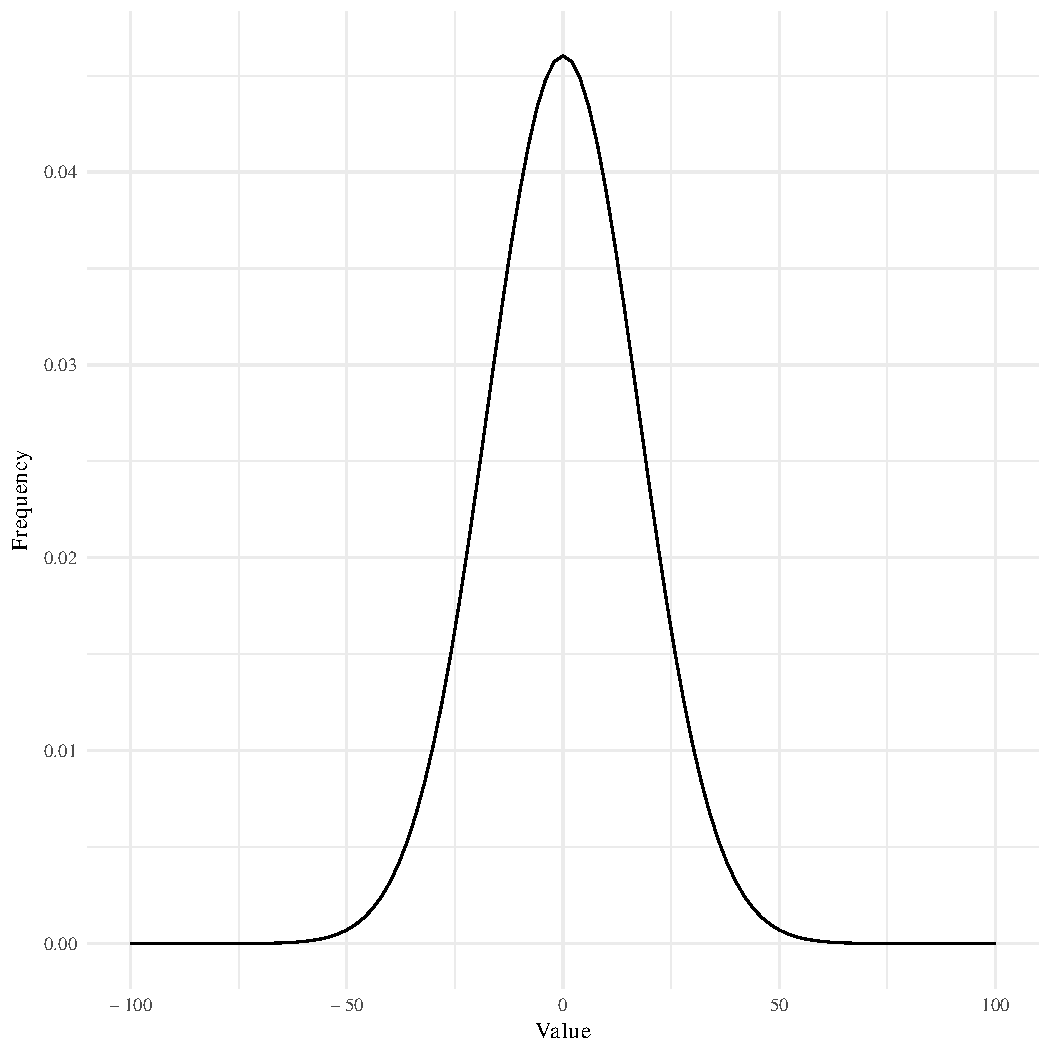
\includegraphics[width=\maxwidth]{figure/unnamed-chunk-7-1} 

\end{knitrout}


\section{Martingale property}

\begin{equation}
\mathop{\mathbb{E}}[X] = \sum_{i=1}^N p_i \times x_i
\end{equation}

To show the martingale property we have to show that the expectation of the symmetric random walk $\mathop{\mathbb{E}}[X|F(0)] = M_0 = 0$

\begin{knitrout}
\definecolor{shadecolor}{rgb}{0.969, 0.969, 0.969}\color{fgcolor}\begin{kframe}
\begin{alltt}
 \hlstd{EM200} \hlkwb{=} \hlkwd{sum}\hlstd{(Mk[}\hlnum{1}\hlopt{:}\hlnum{200}\hlstd{,} \hlnum{200}\hlstd{]} \hlopt{*} \hlstd{fi[}\hlnum{1}\hlopt{:}\hlnum{200}\hlstd{,} \hlnum{200}\hlstd{])} \hlcom{# equal zero.}
\end{alltt}
\end{kframe}
\end{knitrout}

\begin{knitrout}
\definecolor{shadecolor}{rgb}{0.969, 0.969, 0.969}\color{fgcolor}\begin{kframe}
\begin{alltt}
 \hlcom{##}
\hlcom{# Expectation of Mt_l at k}
\hlcom{# denoted by: E[Mt_l|f(k)], with k < l}
\hlcom{##}
\hlcom{##}
\hlcom{# Variables}
\hlcom{##}
\hlstd{from} \hlkwb{<-} \hlnum{2} \hlcom{# Departure of the Expectation}
\hlstd{k} \hlkwb{<-} \hlnum{4} \hlcom{# To get the filtration point }
\hlstd{l} \hlkwb{<-} \hlnum{19} \hlcom{# Give the period to be expected}
\hlkwa{if}\hlstd{(k}\hlopt{>}\hlstd{l)}
\hlstd{interval} \hlkwb{<-} \hlstd{l}\hlopt{-}\hlstd{k}
\hlcom{##}
\hlcom{# Partionated Symmetric Random Walk}
\hlcom{##}
\hlcom{# first the value of M at time $k$ has to be set. It means that the value at this time $k$ is not yet random but resolved.}
\hlcom{# Therefore at time $k$ the variable $M_k$ is not random. }
\hlcom{# We can take any value we want to start with from 1 to $k + 1$.}
\hlcom{# I choose to name this variable $from$:}
\hlstd{from} \hlkwb{<-} \hlnum{2} \hlcom{# Departure of the Expectation}
\hlcom{# The lenght of the path is already know: $(l - k)$:}
\hlstd{len} \hlkwb{<-} \hlstd{l} \hlopt{-} \hlstd{k}
\hlstd{i} \hlkwb{<-} \hlstd{from}\hlopt{:}\hlstd{(from} \hlopt{+} \hlstd{len)}
\hlstd{j} \hlkwb{<-} \hlstd{k}\hlopt{:}\hlstd{l}
\hlstd{df} \hlkwb{<-} \hlstd{Mk[i, j]}
\hlcom{# names(df) <- sapply(1:ncol(df), function(x)\{paste0("X",x)\})}
\hlcom{##}
\hlcom{# Con }
\hlcom{##}

\hlcom{# The probability from k to l start from k to l. The probability table has therefore to be taken from begining.}
\hlstd{fi_min} \hlkwb{<-} \hlstd{fi[}\hlnum{1}\hlopt{:}\hlstd{(len}\hlopt{+}\hlnum{1}\hlstd{),} \hlnum{1}\hlopt{:}\hlstd{(len}\hlopt{+}\hlnum{1}\hlstd{)]}
\hlcom{# Old calculation of fi:}
\hlcom{# }
\hlcom{# fi <- data.frame(matrix(rep(0, (l-k + 1)^2), nrow = l-k + 1))}
\hlcom{# for(j in 1:(l-k+1))}
\hlcom{#   for(i in 1:j)}
\hlcom{#     fi[i, j] <- choose((j-1), (i-1)) * p^(j-1)#((j-1)*p^(j-1))/(factorial(j-1)*factorial(1+i))}
\hlcom{# Finally compute the expectation E[Mt_l|f(k)]:}
\hlstd{Mk[from, k]} \hlopt{==} \hlkwd{sum}\hlstd{(df[, l}\hlopt{-}\hlstd{k}\hlopt{+}\hlnum{1}\hlstd{]} \hlopt{*} \hlstd{fi_min[, l}\hlopt{-}\hlstd{k}\hlopt{+}\hlnum{1}\hlstd{])} \hlcom{#Yeah it is a matringale}
\end{alltt}
\begin{verbatim}
## F(3) 
## TRUE
\end{verbatim}
\end{kframe}
\end{knitrout}

\section{Increments of symmetric random walk}
\begin{equation}
M_{k_{i+1}} - M_{K_i} = \sum_{j = k_{i+1}}^{k_{i+1}} X_j = X_{k_{i+1}}
\end{equation}



\begin{knitrout}
\definecolor{shadecolor}{rgb}{0.969, 0.969, 0.969}\color{fgcolor}\begin{kframe}
\begin{alltt}
\hlcom{# Display the graph:}
\hlstd{SymRandWalk_graph}
\end{alltt}
\end{kframe}
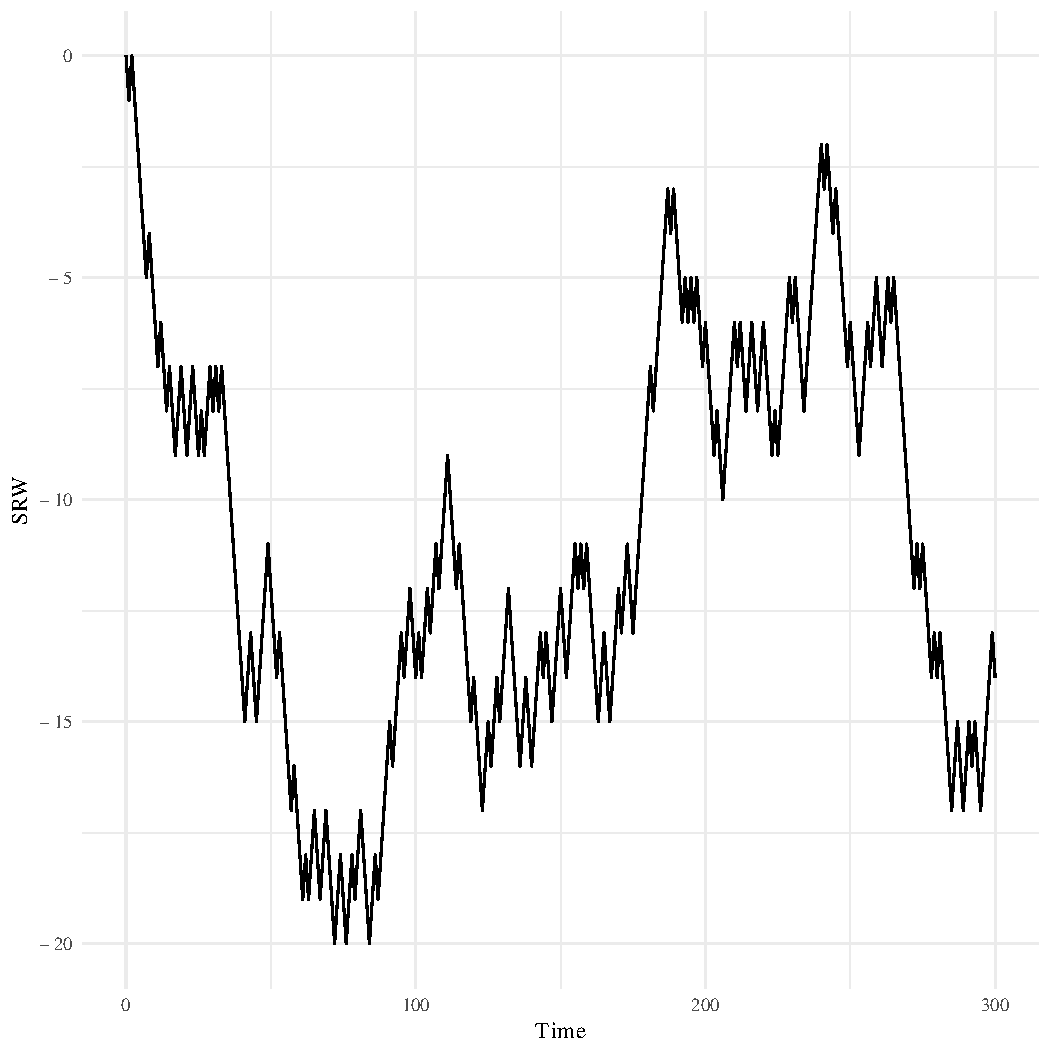
\includegraphics[width=\maxwidth]{figure/unnamed-chunk-10-1} 

\end{knitrout}

The previous graph has the following first 10 increments:

\begin{kframe}
\begin{alltt}
\hlstd{X_tab} \hlkwb{<-} \hlkwd{rbind}\hlstd{(X)}
\hlkwd{colnames}\hlstd{(X_tab)} \hlkwb{<-} \hlkwd{paste0}\hlstd{(}\hlstr{"F("}\hlstd{,} \hlnum{1}\hlopt{:}\hlnum{300}\hlstd{,} \hlstr{")"}\hlstd{)}
\hlkwd{xtable}\hlstd{(X_tab,} \hlkwc{digits} \hlstd{=} \hlnum{0}\hlstd{)}
\end{alltt}
\end{kframe}% latex table generated in R 3.4.0 by xtable 1.8-2 package
% Mon May 22 16:10:57 2017
\begin{table}[ht]
\centering
\begin{tabular}{rrrrrrrrrrrrrrrrrrrrrrrrrrrrrrrrrrrrrrrrrrrrrrrrrrrrrrrrrrrrrrrrrrrrrrrrrrrrrrrrrrrrrrrrrrrrrrrrrrrrrrrrrrrrrrrrrrrrrrrrrrrrrrrrrrrrrrrrrrrrrrrrrrrrrrrrrrrrrrrrrrrrrrrrrrrrrrrrrrrrrrrrrrrrrrrrrrrrrrrrrrrrrrrrrrrrrrrrrrrrrrrrrrrrrrrrrrrrrrrrrrrrrrrrrrrrrrrrrrrrrrrrrrrrrrrrrrrrrrrrrrrrrrrrrrrrrrrrrrrrr}
  \hline
 & F(1) & F(2) & F(3) & F(4) & F(5) & F(6) & F(7) & F(8) & F(9) & F(10) & F(11) & F(12) & F(13) & F(14) & F(15) & F(16) & F(17) & F(18) & F(19) & F(20) & F(21) & F(22) & F(23) & F(24) & F(25) & F(26) & F(27) & F(28) & F(29) & F(30) & F(31) & F(32) & F(33) & F(34) & F(35) & F(36) & F(37) & F(38) & F(39) & F(40) & F(41) & F(42) & F(43) & F(44) & F(45) & F(46) & F(47) & F(48) & F(49) & F(50) & F(51) & F(52) & F(53) & F(54) & F(55) & F(56) & F(57) & F(58) & F(59) & F(60) & F(61) & F(62) & F(63) & F(64) & F(65) & F(66) & F(67) & F(68) & F(69) & F(70) & F(71) & F(72) & F(73) & F(74) & F(75) & F(76) & F(77) & F(78) & F(79) & F(80) & F(81) & F(82) & F(83) & F(84) & F(85) & F(86) & F(87) & F(88) & F(89) & F(90) & F(91) & F(92) & F(93) & F(94) & F(95) & F(96) & F(97) & F(98) & F(99) & F(100) & F(101) & F(102) & F(103) & F(104) & F(105) & F(106) & F(107) & F(108) & F(109) & F(110) & F(111) & F(112) & F(113) & F(114) & F(115) & F(116) & F(117) & F(118) & F(119) & F(120) & F(121) & F(122) & F(123) & F(124) & F(125) & F(126) & F(127) & F(128) & F(129) & F(130) & F(131) & F(132) & F(133) & F(134) & F(135) & F(136) & F(137) & F(138) & F(139) & F(140) & F(141) & F(142) & F(143) & F(144) & F(145) & F(146) & F(147) & F(148) & F(149) & F(150) & F(151) & F(152) & F(153) & F(154) & F(155) & F(156) & F(157) & F(158) & F(159) & F(160) & F(161) & F(162) & F(163) & F(164) & F(165) & F(166) & F(167) & F(168) & F(169) & F(170) & F(171) & F(172) & F(173) & F(174) & F(175) & F(176) & F(177) & F(178) & F(179) & F(180) & F(181) & F(182) & F(183) & F(184) & F(185) & F(186) & F(187) & F(188) & F(189) & F(190) & F(191) & F(192) & F(193) & F(194) & F(195) & F(196) & F(197) & F(198) & F(199) & F(200) & F(201) & F(202) & F(203) & F(204) & F(205) & F(206) & F(207) & F(208) & F(209) & F(210) & F(211) & F(212) & F(213) & F(214) & F(215) & F(216) & F(217) & F(218) & F(219) & F(220) & F(221) & F(222) & F(223) & F(224) & F(225) & F(226) & F(227) & F(228) & F(229) & F(230) & F(231) & F(232) & F(233) & F(234) & F(235) & F(236) & F(237) & F(238) & F(239) & F(240) & F(241) & F(242) & F(243) & F(244) & F(245) & F(246) & F(247) & F(248) & F(249) & F(250) & F(251) & F(252) & F(253) & F(254) & F(255) & F(256) & F(257) & F(258) & F(259) & F(260) & F(261) & F(262) & F(263) & F(264) & F(265) & F(266) & F(267) & F(268) & F(269) & F(270) & F(271) & F(272) & F(273) & F(274) & F(275) & F(276) & F(277) & F(278) & F(279) & F(280) & F(281) & F(282) & F(283) & F(284) & F(285) & F(286) & F(287) & F(288) & F(289) & F(290) & F(291) & F(292) & F(293) & F(294) & F(295) & F(296) & F(297) & F(298) & F(299) & F(300) \\ 
  \hline
X & -1 & 1 & -1 & -1 & -1 & -1 & -1 & 1 & -1 & -1 & -1 & 1 & -1 & -1 & 1 & -1 & -1 & 1 & 1 & -1 & -1 & 1 & 1 & -1 & -1 & 1 & -1 & 1 & 1 & -1 & 1 & -1 & 1 & -1 & -1 & -1 & -1 & -1 & -1 & -1 & -1 & 1 & 1 & -1 & -1 & 1 & 1 & 1 & 1 & -1 & -1 & -1 & 1 & -1 & -1 & -1 & -1 & 1 & -1 & -1 & -1 & 1 & -1 & 1 & 1 & -1 & -1 & 1 & 1 & -1 & -1 & -1 & 1 & 1 & -1 & -1 & 1 & 1 & -1 & 1 & 1 & -1 & -1 & -1 & 1 & 1 & -1 & 1 & 1 & 1 & 1 & -1 & 1 & 1 & 1 & -1 & 1 & 1 & -1 & -1 & 1 & -1 & 1 & 1 & -1 & 1 & 1 & -1 & 1 & 1 & 1 & -1 & -1 & -1 & 1 & -1 & -1 & -1 & -1 & 1 & -1 & -1 & -1 & 1 & 1 & -1 & 1 & 1 & -1 & 1 & 1 & 1 & -1 & -1 & -1 & -1 & 1 & 1 & -1 & -1 & 1 & 1 & 1 & -1 & 1 & -1 & -1 & 1 & 1 & 1 & -1 & -1 & 1 & 1 & 1 & -1 & 1 & -1 & 1 & -1 & -1 & -1 & -1 & 1 & 1 & -1 & -1 & 1 & 1 & 1 & -1 & 1 & 1 & -1 & -1 & 1 & 1 & 1 & 1 & 1 & 1 & -1 & 1 & 1 & 1 & 1 & 1 & -1 & 1 & -1 & -1 & -1 & 1 & -1 & 1 & -1 & 1 & -1 & -1 & 1 & -1 & -1 & -1 & 1 & -1 & -1 & 1 & 1 & 1 & 1 & -1 & 1 & -1 & -1 & 1 & 1 & -1 & -1 & 1 & 1 & -1 & -1 & -1 & 1 & -1 & 1 & 1 & 1 & 1 & -1 & 1 & -1 & -1 & -1 & 1 & 1 & 1 & 1 & 1 & 1 & -1 & 1 & -1 & -1 & 1 & -1 & -1 & -1 & -1 & 1 & -1 & -1 & -1 & 1 & 1 & 1 & -1 & 1 & 1 & -1 & -1 & 1 & 1 & -1 & 1 & -1 & -1 & -1 & -1 & -1 & -1 & -1 & 1 & -1 & 1 & -1 & -1 & -1 & 1 & -1 & 1 & -1 & -1 & -1 & -1 & 1 & 1 & -1 & -1 & 1 & 1 & -1 & 1 & -1 & -1 & 1 & 1 & 1 & 1 & -1 \\ 
   \hline
\end{tabular}
\end{table}



\subsection{Expectation and Variance of increments}

\begin{equation}
\mathop{\mathbb{E}}[X_j] = 0 \Rightarrow \mathop{\mathbb{E}}[M_{k_{i+1}} - M_{k_i}] = 0
\end{equation}

\begin{equation}
Var(M_{k_{i+1}}) - M_{k_i}) = k_{i+1} - K_i
\end{equation}

\begin{knitrout}
\definecolor{shadecolor}{rgb}{0.969, 0.969, 0.969}\color{fgcolor}\begin{kframe}
\begin{alltt}
\hlcom{# Xk is the possible outcome of the random variable X:}
\hlstd{Xk} \hlkwb{<-} \hlkwd{c}\hlstd{(}\hlnum{1}\hlstd{,} \hlopt{-}\hlnum{1}\hlstd{)}
\hlcom{# Expectation:}
\hlstd{Ex} \hlkwb{<-} \hlkwd{weighted.mean}\hlstd{(Xk,} \hlkwd{c}\hlstd{(p, q))}
\hlstd{Ex.square} \hlkwb{<-} \hlkwd{weighted.mean}\hlstd{(Xk}\hlopt{^}\hlnum{2}\hlstd{,} \hlkwd{c}\hlstd{(p, q))}
\hlcom{# Variance}
\hlstd{S} \hlkwb{<-} \hlstd{Ex.square} \hlopt{-} \hlstd{Ex}\hlopt{^}\hlnum{2}
\end{alltt}
\end{kframe}
\end{knitrout}

To find the variance the following formula has been used:
\begin{equation}
\begin{array}{lll}
Var(X) & = & \mathop{\mathbb{E}}(X - \mu)^2 \\
& = & \mathop{\mathbb{E}}X^2 + \mu^2 - 2\mu^2 = \mathop{\mathbb{E}}X^2 - \mu^2
\end{array}
\end{equation}

   
\end{document}





















